\documentclass[conference]{IEEEtran}

\usepackage{cite}
\usepackage{amsmath,amssymb,amsfonts}
\usepackage{graphicx}
\usepackage{listings}
\usepackage{url}
\def\UrlBreaks{\do\/\do-}
\Urlmuskip=0mu plus 1mu\relax

\lstdefinestyle{fstar}{
  basicstyle=\scriptsize\ttfamily,
  breaklines=true,
  columns=fullflexible,
  frame=single,
  float,
  floatplacement=tbp,
  keepspaces=true,
  showstringspaces=false,
  captionpos=b
}

\def\BibTeX{{\rm B\kern-.05em{\sc i\kern-.025em b}\kern-.08em
    T\kern-.1667em\lower.7ex\hbox{E}\kern-.125emX}}

\begin{document}

\title{Proof-Oriented Validation of LLM-Generated Intents for Autonomous Networks}

% ICNP 2026 currently uses double-blind review. Replace this block for camera-ready.
\author{\IEEEauthorblockN{Anonymous Submission}}

\maketitle

\begin{abstract}
Natural language (NL) intents will be increasingly the control mechanism of 5G/6G autonomous telecom networks.

Example intent: ``\textit{Provide an ultra-reliable low-latency 5G service for telemedicine and critical care operations at Mayo Clinic on an ongoing basis. Support up to 80 critical devices and 200 auxiliary endpoints. Maintain end-to-end latency below 10 ms \ldots}''

This shift creates a safety and reliability problem: natural-language or weakly structured intents are attractive at the management plane, but they can be ambiguous, under-specified, and may not validate against additional provider-specific operational constraints.

This paper presents a prototype, high-assurance, intent-admission shell for autonomous networks built around the TM Forum TMF921 Intent Management API which serves as ``front door'' for NL intents and as such imposes the minimal semantic requirements through an OWL ontology. However any specific telecom provider implementation of TMF921 will have additional requirements that are not covered by the ontology.

This paper shows how natural-language intents can be trusted through proof-relevant guarantees provided by formal verification systems based on dependently typed languages. First (offline) the OWL ontology is converted to the equivalent dependent types of the F* language. These serve as propositions against which incoming intents may be checked. Then (online) received natural-language intents are translated by a Large Language Model (LLM) to F* code that is validated (type-checked) against the ontology-derived dependent types, by the F* proof checker. Only valid intents are admitted.

Further, since TMF921 structure-imposition is necessarily generic, we demo provider-specific intent validation via further refinements of the ontology types.

It is observed that valid intents are almost always correctly processed. Specifically, the LLM (GPT-5.4) produces correct F* code in approximately 99\% of cases on the first attempt, and achieves 100\% correctness with a single retry. These results suggest that the apparent non-determinism of natural language and LLM-generated outputs can be effectively mitigated through dependent-type-based validation.
\end{abstract}

\begin{IEEEkeywords}
autonomous networks, large language models, formal verification, dependent types, intent admission
\end{IEEEkeywords}

\section{Introduction}

Autonomous networks are a particularly demanding instance of a broader systems problem: humans and software agents can easily generate natural language requests, but fluent output is not the same as safe or correct output. Similar boundary problems already appear in configuration validation \cite{ciri}, natural-language firewall configuration \cite{firewall_nl}, and production multi-agent network management \cite{confucius}. Recent agent-security work argues that systems should apply defense-in-depth and complete mediation rather than treat model outputs as trustworthy by default \cite{security_principles}. This concern is particularly acute for network control workflows where accepted requests can eventually influence provisioning, routing, or remediation.

At this boundary, two distinct sources of non-determinism must be controlled. The first is the natural-language request itself -- the same meaning can be conveyed in different surface forms. The second is the LLM-generated artifact used to interpret that request, whose output may vary across runs even when the intended meaning is unchanged. Proof-checked output validation counters both by accepting only interpretations that can be turned into the required machine-checkable artifact.

This paper describes a prototype shell around the TM Forum \cite{tmforum_site} TMF921 Intent Management API \cite{tmf921_api_page} that addresses this admission problem. TM921 allows for intent submission in natural language, structured JSON, or weakly structured JSON formats. Here the focus is on the natural-language path.

First, offline, the TM Forum intent ontology is projected into F* dependent types that capture the standards-aligned semantics of the API \cite{tr290a,tr292d,fstar_site,fstar_popl}. Then, online, incoming requests at the TM921 boundary are normalized and, for the natural-language path, translated by an LLM into F* artifacts that must type-check against that ontology-derived layer before admission. Around that checked path, the system emits a canonical intent intermediate representation (IR), normalized JSON-LD, generated F* modules and other items for traceability and diagnostics.

Our argument is not that formal methods alone solve autonomous-network safety, nor that natural-language interfaces should be avoided. Instead, we argue for a narrow and practical claim: the boundary between LLM generation and provider execution is the right place to combine standards-aligned API handling, semantic normalization, and machine-checked admissibility tests. Autonomous networking is the motivating domain here, but the pattern applies more generally wherever model-generated artifacts must be highly trusted before they can allocate resources, change policy, or trigger control-plane actions.

\subsection{Contributions}

This paper makes two main contributions:
\begin{enumerate}
\item It frames dependent-type, proof-oriented validation as an admission-layer pattern for high-trust LLM outputs and instantiates that pattern as a TMF921 compliant API \cite{tmf921_spec,tr292_tio}.
\item It separates general intent validity from provider-specific admissibility, allowing failures such as under-specification, infeasible requests, and policy violations to be localized. This is achieved by successively refining the dependent types derived from the TM Forum ontology, to provider-specific types. This system allows different providers to use the same standards-aligned core while layering on their own constraints.
\end{enumerate}

\section{Dependent Types and Proof-Oriented Validation}

Via the Curry--Howard correspondence \cite{propositions_as_types}, propositions can be represented as types and proofs as programs; in our setting, we encode the required intent obligations as F* types. Then, the LLM-generated artifact (\textit{the program}) is a candidate proof of those types. Successful type checking serves as machine-checked evidence of compliance. Practical proof-oriented systems such as Lean \cite{lean_theorem_prover} and F* \cite{fstar_popl} make this style of checked construction usable for real systems.

To illustrate, consider a simple function type \texttt{T1} given in Listing~\ref{lst:simple-function}, whose inputs and outputs are natural numbers. 

\begin{lstlisting}[style=fstar,caption={Simple function type in F*.},label={lst:simple-function}]
//declare a function type that takes a nat and returns a nat
type T1 = nat -> nat  

//this function satisfies type T1 (as would many others)
let addOne: T1 =  fun x -> x + 1  
\end{lstlisting}

Since \texttt{T1} is \textit{inhabited} via the function \texttt{addOne} it means that \texttt{addOne} is a proof of \texttt{T1}. So under Curry--Howard the type \texttt{T1} can be read as a proposition that is proven by the program \texttt{addOne}.

Now lets consider a slightly more complex function type that accepts and returns even numbers. We can express this using dependent types given in Listing~\ref{lst:dependent-function}. Here, \texttt{Even n} is a dependent type that represents the proposition that a natural number is even. Subsequently, the function type \texttt{T2} requires that inputs and outputs should be of type \texttt{Even n}. 

\begin{lstlisting}[style=fstar,caption={More complex dependent function type in F*.},label={lst:dependent-function}]
//first define a dependent type for even numbers 
//as a constraint on nat
type Even (n:nat) = _:unit { n % 2 = 0 } 

//then define a dependent function type that 
//requires Even input and output
type T2 = (x: nat{Even x}) -> nat{Even result}  

//this function satisfies type T2 because it takes an 
//even number and produces an even number
let addTwo: T2 = fun x -> x + 2  

//this function does NOT satisfy type T2 because it 
//takes an even number but produces an odd number
let addOneError: T2 = fun x -> x + 1  
\end{lstlisting}

The type \texttt{Even n} is a dependent type because it \textit{depends} on the \textit{value} \texttt{n} which is supplied from where the type is used. Here \texttt{n} in \texttt{Even n} is used in the constraint \texttt{n \% 2 = 0} that is part of the type declaration. In fact any arbitrary constraint can be used as part of a type declaration.
\textit{To surmise, in a dependent type system, types can depend on values and other functions}. However, this simple explanation does not do justice to the full expressiveness of dependent types, but it gives a flavor of how they can encode constraints. 

Suffice is to understand is that a complex set of constraints can be encoded as a dependent types. Even state-machines can be encoded as types. The key point is that system (or business) constraints/rules can be \textit{modelled} as types. Then, the validation (of code that uses these types) is automatic via the proof-oriented type checkers. Non-dependently typed languages -- with simpler type checkers -- cannot express such constraints as types.

Once the systems/business rules are modelled as types, then LLM-generated \textit{programs} can be validated against them, thus eliminating the source of non-determinism inherent with LLM-generated outputs.

\section{The Unreasonable Effectiveness of Dependent Types}
Experiments show that current \textit{frontier} models can produce correct F* code most of the time on the first attempt, which was far less plausible in the late-2024 GPT-4o/o1 period. Table~\ref{tab:gpt54-gpt4o} compares GPT-5.4 and GPT-4o using only benchmarks that appear under the same name in official OpenAI sources. The overlap is limited, but the shared results still indicate a substantial recent increase in reasoning and agentic reliability. The same trend is reflected in the emergence and rise of dedicated agentic coding products such as Anthropic's Claude Code \cite{claude_code_overview}, OpenAI's Codex \cite{codex_openai}, and GitHub Copilot \cite{github_copilot_features}.

A plausible contributor to this improvement is the broader shift toward reinforcement learning with verifiable rewards (RLVR) \cite{rlvr_grpo} on tasks with objective checkers, including mathematics, code, and formal reasoning. Public evidence for proprietary \textit{frontier} models remains limited. However, Google DeepMind states that the advanced Gemini Deep Think model used for International Mathematical Olympiad (IMO)-level reasoning \cite{imo_official} was additionally trained with novel reinforcement learning techniques that leverage multi-step reasoning, problem-solving, and theorem-proving data \cite{gemini_deep_think_imo}. In the open literature, Tulu 3 explicitly identifies RLVR as a post-training method \cite{tulu3_rlvr}, and recent Lean-based work shows how proof assistants can serve as verifier-grounded reward oracles during theorem-proving training \cite{process_verified_rl_lean}. While these sources do not establish that GPT-5.4 itself was post-trained on Lean traces, they do show that verifiable-reward training over formal reasoning tasks is now a credible part of the broader frontier-model toolkit.

The likely involvement of dependently-typed languages in post-training of frontier LLMs (either directly or indirectly) is an indication towards their satisfactory performance on dependent-type code generation.

\begin{table}[t]
\centering
\caption{Official OpenAI-reported results on benchmarks with exact name overlap between GPT-4o and GPT-5.4 \cite{gpt54_openai,gpt41_openai,browsecomp_openai}.}
\label{tab:gpt54-gpt4o}
\begin{tabular}{lcc}
\hline
Benchmark & GPT-4o & GPT-5.4 \\
\hline
GPQA Diamond & 46.0\% & 92.8\% \\
BrowseComp & 1.9\% & 82.7\% \\
\hline
\end{tabular}

\parbox{0.95\linewidth}{\footnotesize \textit{Note:} The BrowseComp entry uses the browsing-enabled GPT-4o result reported by OpenAI, since GPT-5.4 was evaluated on BrowseComp with ChatGPT search enabled.}
\end{table}

\section{Processing Overview}

The prototype shell implementation has two distinct stages offline and online. Offline, a selected subset of the TM Forum intent ontology is projected into F* modules that define the standards-aligned baseline used by the checker \cite{tr292_tio,tr290a,tr292d,fstar_site,fstar_popl}. Online, the TM921 \textit{expression} field is extracted, translated into F* artifacts when needed, and admitted only if both standards-aligned and provider-specific predicates hold. Additional artifacts are also emitted for traceability and diagnostics.

Figure~\ref{fig:processing-pipeline} summarizes this online path and shows where rejection diagnostics are produced.

\begin{figure}[t]
\centering
\begingroup
\footnotesize
\setlength{\fboxsep}{4pt}
\renewcommand{\arraystretch}{1.15}
\newcommand{\admissionflowbox}[2]{\fbox{\begin{minipage}{#1}\centering #2\end{minipage}}}
\newcommand{\admissionmainbox}[1]{\admissionflowbox{0.57\linewidth}{#1}}
\newcommand{\admissionsidebox}[1]{\admissionflowbox{0.27\linewidth}{#1}}
\begin{tabular}{@{}c@{\hspace{0.35em}}c@{\hspace{0.35em}}c@{}}
\admissionmainbox{\textbf{TMF921 Web API}\\request received} & & \\
$\Downarrow$ & & \\
\admissionmainbox{\textbf{Classify request}\\natural language, structured JSON, or ambiguous}
& $\Rightarrow$ &
\admissionsidebox{\textbf{Reject}\\ambiguous request diagnostics} \\
$\Downarrow$ & & \\
\admissionmainbox{\textbf{Normalize or translate}\\canonical/normalizable $\rightarrow$ canonical representation\\natural language $\rightarrow$ LLM-generated F*}
& & \\
$\Downarrow$ & & \\
\admissionmainbox{\textbf{Ontology type check}\\F* checked against TM Forum ontology-derived dependent types}
& $\Rightarrow$ &
\admissionsidebox{\textbf{Reject}\\under-specified or semantically invalid} \\
$\Downarrow$ & & \\
\admissionmainbox{\textbf{Standards-aligned admission}\\emit JSON-LD, F* modules, diagnostics, and hashes}
& & \\
$\Downarrow$ & & \\
\admissionmainbox{\textbf{Provider refinements}\\capacity, latency, policy, and reporting checks}
& $\Rightarrow$ &
\admissionsidebox{\textbf{Reject}\\provider-specific diagnostics} \\
$\Downarrow$ & & \\
\admissionmainbox{\textbf{Accepted intent}\\available for downstream orchestration} & &
\end{tabular}
\endgroup
\caption{Online TMF921 intent-admission pipeline. The standards-aligned gate checks whether the request is actionable under the ontology-derived dependent types; provider refinements then check local admissibility constraints.}
\label{fig:processing-pipeline}
\end{figure}

\section{Example Ontology Fragment and Refinement}
To illustrate the projection and refinement process, consider a live-broadcast scenario family with the following sample request: 

\par\indent ``\textit{Provide a premium 5G broadcast service for the live event at Detroit Stadium on April 25, 2026 from 18:00 to 22:00 EST. Support up to 200 production devices. Keep uplink latency under 20 ms. Send hourly compliance updates and immediate alerts if service quality degrades. Do not impact emergency-service traffic.}''

Figure~\ref{fig:ontology-fragment} shows the compact ontology fragment used to interpret this request. The fragment is intentionally small: an intent has a target, a service class, a delivery window, measurable quantities, a reporting expectation, and a safety or security posture. For the live-broadcast scenario, these fields are enough to distinguish a vague request from an actionable intent without exposing the reader to the full ontology.

\begin{figure}[t]
\centering
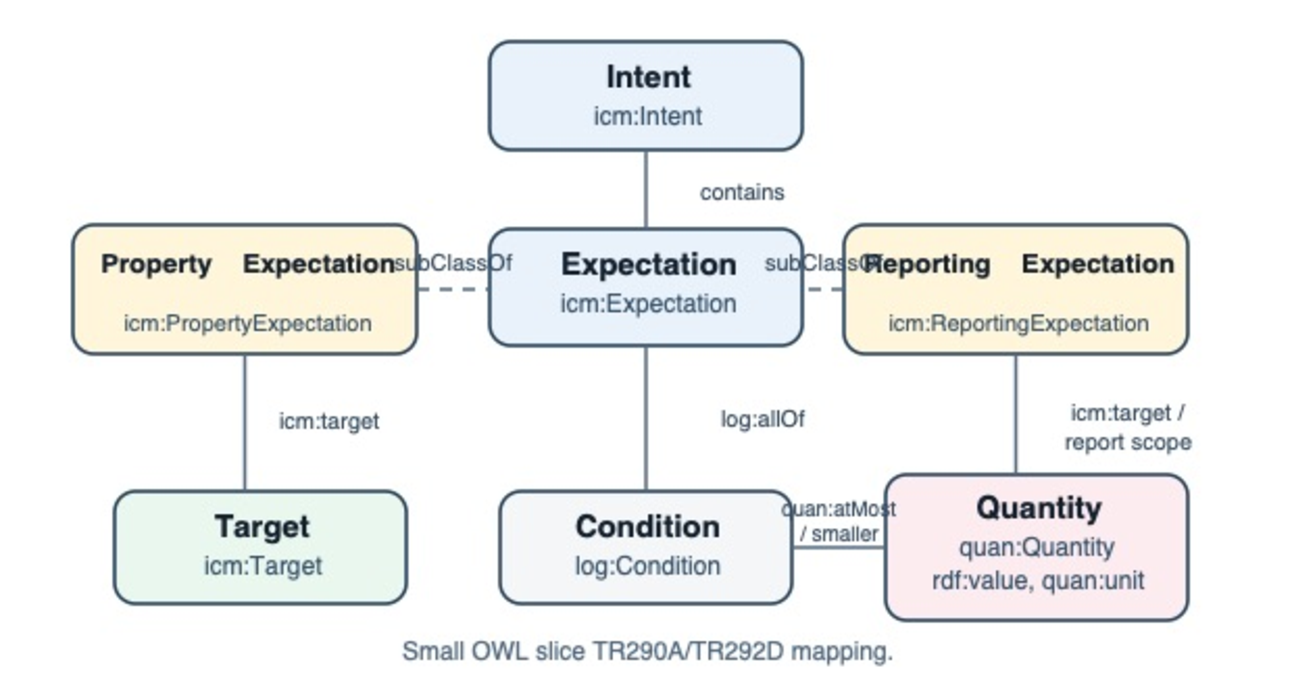
\includegraphics[width=\linewidth]{tr290a_tr292d_fragment.pdf}
\caption{Simplified class-level fragment used by the case study; adapted from TR290A Sections 2, 4, 5, 8, and 9 \cite{tr290a} and TR292D Sections 2 and 5 \cite{tr292d}. TM921 provides the expression envelope used to carry this ontology content over the API \cite{tmf921_spec}.}
\label{fig:ontology-fragment}
\end{figure}

The first projection turns the standards-aligned fragment into common-core F* predicates. Listing~\ref{lst:common-core} elides record fields and helper definitions, but shows the important shape: the request must name a target and service, provide a complete window and reporting expectation, and attach positive measurable quantities.

\begin{lstlisting}[style=fstar,caption={Simplified common-core F* excerpt derived from the ontology fragment.},label={lst:common-core}]
let measurable (i:raw_tm_intent) : bool =
  target_present (target_descriptor_of i) &&
  service_present i.service_class &&
  delivery_window_present (delivery_window_of i) &&
  reporting_expectation_present
    (reporting_expectation_of i) &&
  required_metrics_present
    (requires_auxiliary_metric i)
    (metric_requirements_of i)

let quantities_ok (i:raw_tm_intent) : bool =
  all_quantities_positive (requires_auxiliary_metric i)
    (primary_device_quantity_of i)
    (auxiliary_endpoint_quantity_of i)
    (max_latency_quantity_of i)
    (reporting_interval_quantity_of i)

let common_core_valid i =
  measurable i && quantities_ok i
\end{lstlisting}

Provider checks are then layered on top of the common core. In the running live-broadcast example, Detroit Stadium resolves to the \texttt{LiveBroadcastGold} profile, which admits at most 250 production devices and requires a latency bound no tighter than 20 ms. The accepted scenario requests 200 devices, 20 ms uplink latency, hourly reporting, 
immediate degradation alerts, and no emergency-traffic preemption.

\begin{lstlisting}[style=fstar,caption={Simplified provider refinement excerpt for live broadcast admission.},label={lst:provider-refinement}]
type profile =
  | LiveBroadcastSilver
  | LiveBroadcastGold
  | UnsupportedProfile

let resolve_profile i =
  match i.scenario_family,
        (target_descriptor_of i).descriptor_name with
  | BroadcastFamily, Some "Detroit Stadium" ->
      LiveBroadcastGold
  | BroadcastFamily, Some "Metro Arena" ->
      LiveBroadcastSilver
  | _ -> UnsupportedProfile

let provider_valid p i =
  common_core_valid i && profile_matches p i &&
  capacity_ok p i && latency_ok p i &&
  policy_ok i

type provider_checked_intent (p:profile) (i:raw_tm_intent) =
  v:raw_tm_intent{ v == i /\ provider_valid p v }
\end{lstlisting}

This witness structure localizes failures. A request missing a target, window, or quantity cannot construct the common-core witness; a request with excessive device count, an impossible latency claim, or public-safety preemption can pass the ontology-derived gate and still fail the provider witness. This is the separation between general intent validity and local provider admissibility.

\section{Admission Boundary and Validation}

The TM921 shell treats every submission as a candidate intent rather than executable authority. Inputs are classified as canonical, normalizable, natural language, or ambiguous; admitted inputs are lowered into a canonical IR that records proof-relevant fields and source provenance. This typed interposition is aligned with prior work on typed IRs and safety gates for LLM-assisted systems \cite{firewall_nl,mtp,ciri}, and operationalizes complete mediation at the intent boundary \cite{security_principles}. In the case study, the shell also compares the proof-oriented checks against a repo-local JSON Schema baseline so that the value of the typed admission lane is visible rather than assumed.

As illustrated in Fig.~\ref{fig:ontology-fragment} and Listings~\ref{lst:common-core}--\ref{lst:provider-refinement}, the admission model has two gates. The first asks whether the request is specific enough to count as an actionable intent at all: it must contain the proof-relevant structure, measurable quantities, and temporal context required by the selected TR290A/TR292D subset \cite{tr290a,tr292d}. The second applies provider-specific refinements such as capacity, latency, reporting, and traffic-protection constraints \cite{tr292_tio,tr292i}. This separation matters because it distinguishes requests that are not real intents from requests that are real intents but unsafe to enact.

The shell also retains sidecar evidence so that acceptance and rejection remain auditable \cite{security_principles,ciri,confucius}. This evidence includes:
\begin{itemize}
\item the canonical intermediate representation (IR),
\item normalized JSON-LD,
\item generated F* modules, and
\item checker diagnostics.
\end{itemize}

\section{Prototype and Case Study}

The prototype is implemented as Web API service (written in F\# \cite{fsharp}) with F* models for checked scenarios \cite{fstar_site,fstar_popl}. The current case study uses live-broadcast service requests and performs two levels of validation:
\begin{itemize}
\item base checks against the TM Forum ontology-derived dependent types, and
\item provider-specific checks with further refined types.
\end{itemize}

The scenario family includes one success path, several provider-side failures such as invalid window, excessive capacity, unrealistic latency, and policy violations, a profile-sensitive acceptance/rejection pair, and an under-specified request. 

The study is illustrative rather than a large-scale benchmark, but it shows the value of treating LLM output as a candidate artifact that must cross a machine-checked admission boundary.

\section{Discussion}

The main systems point is simple: LLM output should be treated as a candidate intent, not as executable authority. In autonomous networks, this provides a bounded-autonomy control point before provisioning or remediation. More broadly, it is one practical way to enforce defense-in-depth and complete mediation for high-trust agent outputs \cite{security_principles}.

TMF921 and TIO make the network instantiation concrete because they provide a standards-aligned API and semantic baseline \cite{tmf921_spec,tr292_tio}. But the pattern does not depend on telecom specifics. Any domain with a typed admissibility model and local refinement predicates can apply the same structure \cite{firewall_nl,ciri,confucius}.

\section{Limitations and Future Work}

The current evidence is architectural rather than broad empirical. The natural-language handling is narrow, the provider model is simplified, and the evaluation covers a single scenario family. The next steps are to broaden the scenario set, connect admission checks to dynamic state, and compare proof-oriented admission more systematically against lighter-weight baselines.

\section{Related Work}

Prior work already points toward validated intermediate artifacts for LLM-assisted systems. Ciri studies output checking for configuration validation \cite{ciri}, while Taghiyev and Aslanbayli use natural language only to produce a typed IR for firewall rules \cite{firewall_nl}. Meaning-Typed Programming similarly argues for semantically structured intermediate representations in LLM-integrated applications \cite{mtp}. Our work follows the same direction, but emphasizes proof-oriented admissibility at the execution boundary.

On the safety side, Zhang et al. argue that LLM agents should adopt classic security principles such as defense-in-depth and complete mediation \cite{security_principles}. In networking, the Confucius framework shows that multi-agent systems already rely on validation layers and existing tooling to reduce regressions \cite{confucius}. Our contribution is complementary: we focus on the earlier boundary where candidate requests first become eligible for authoritative handling.

\section{Conclusion}

This paper argues that the admission boundary is the right place to enforce high assurance over LLM-generated intents. In the TMF921 case study, natural-language or weakly structured requests are treated as candidate intents, normalized into a canonical IR, and admitted only when the corresponding F* artifacts satisfy standards-aligned and provider-specific predicates.

The broader lesson is that highly trusted AI outputs should not be trusted because they are fluent. They should be trusted only after they cross a machine-checked admission boundary that makes their semantics explicit, their constraints auditable, and their right to trigger downstream action conditional on proof-oriented validation.

\bibliographystyle{IEEEtran}
\bibliography{icnp2026_submission}

\end{document}
